\documentclass{standalone}
\usepackage{tikz}
\usetikzlibrary{calc}
\usetikzlibrary{shapes,arrows,positioning,decorations.pathreplacing}
\usepackage{amsmath}


\tikzset{
  mystyle/.style={draw=none}
}

\begin{document}
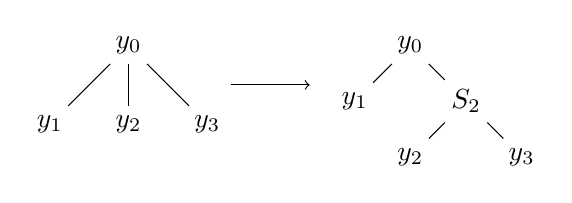
\begin{tikzpicture}[node distance=1cm]
    
    \node(y0)[mystyle]{$y_0$};
    \node(y2)[mystyle, below of = y0]{$y_2$};
    \node(y1)[mystyle, left of = y2]{$y_1$};
    \node(y3)[mystyle, right of = y2]{$y_3$};
    % \node(start)[mystyle]{Start};
    \draw (y0) edge (y1);
    \draw (y0) edge (y2);
    \draw (y0) edge (y3);

    % \rightarrow
    \draw[->] (1.3, -0.5) -- (2.3, -0.5);

    \node(y0r)[mystyle, right = 3cm of y0]{$y_0$};
    % \node(y2r)[mystyle, below left of = y0]{$y_2$};
    \node(y1r)[mystyle, below left of = y0r]{$y_1$};
    \node(s2r)[mystyle, below right of = y0r]{$S_2$};
    \node(y2r)[mystyle, below left of = s2r]{$y_2$};
    \node(y3r)[mystyle, below right of = s2r]{$y_3$};
    % \node(y3r)[mystyle, right of = y2]{$y_3$};
    % \node(start)[mystyle]{Start};
    \draw (y0r) edge (y1r);
    \draw (y0r) edge (s2r);
    \draw (s2r) edge (y2r);
    \draw (s2r) edge (y3r);
    % \draw (y0) edge (y2);
    % \draw (y0) edge (y3);
    
\end{tikzpicture}
\end{document}
